\documentclass[a4paper,12pt]{article}
\usepackage[utf8]{inputenc}
\usepackage{amsmath}
\usepackage{amsfonts}
\usepackage{amssymb}
\usepackage{graphicx}
\usepackage{caption}
\usepackage{subcaption}
\usepackage{float}
\usepackage{siunitx}
\usepackage{booktabs}
\usepackage{hyperref}
\usepackage{titling}

\title{Analisi circuiti Inverter e NOR RTL}
\author{Francesco Giuseppe Minisini}
\date{\today}

\begin{document}
\maketitle
\hrule
\vspace{9pt}
\begin{abstract}
    % Nelle seguenti esperienze di laboratorio sono stati realizzati su "breadboard" circuiti di tipologia Inverter RTL, NOR RTL, NAND RTL e ne si è studiato il comportamento nel dominio del tempo e rilevandone, tramite oscilloscopio, l'andamento nel tempo del segnale di tensione in uscita $v_{out}(t)$ sottoponendo i circuiti a configurazioni di segnali in ingresso $v_{in}(t)$ differenti, in modo da confrontare le misure ottenute con i risultati previsti dall'analisi teorica e da simulazioni eseguite tramite "LTspice". L'esprienza si è poi concentrata nella misurazione di grandezze caratteristiche del circuito Inverter RTL sia in discesa che in salita, come il tempo di ritardo \(t_{deley}^{discesa} = \pm s\) e \(t_{deley}^{salita} = \pm s\) e il tempo di discesa e salita in uscita \(t_{uscita}^{discesa}= \pm s\) e \(t_{uscita}^{discesa}= \pm s\). 
    Nelle seguenti esperienze di laboratorio sono stati realizzati su breadboard circuiti di tipologia Inverter RTL e NOR RTL. Ne è stato studiato il comportamento nel dominio del tempo, rilevando tramite oscilloscopio l’andamento nel tempo del segnale di tensione in uscita \(v_{out}(t)\), sottoponendo i circuiti a diverse configurazioni di segnali in ingresso \(v_{in}(t)\). Le misure sperimentali sono state confrontate con i risultati teorici attesi e con simulazioni effettuate tramite software LTspice.
    L’analisi si è concentrata in particolare sul circuito Inverter RTL, del quale sono stati misurati i seguenti parametri dinamici: il tempo di ritardo in discesa \(t_{df} = (80 \pm 10)\,\mathrm{ns}\), il tempo di discesa \(t_f = (80 \pm 10)\,\mathrm{ns}\), il tempo di ritardo in salita \(t_{dr} = (2.10 \pm 0.10)\,\mu\mathrm{s}\), e il tempo di salita \(t_r = (420 \pm 10)\,\mathrm{ns}\) e il livello logico \(V_{OL} = (41 \pm 4)\,\mathrm{mV}\). 
    % Sono inoltre stati determinati i livelli logici: \(V_{OH} = (5.000 \pm 0.004)\,\mathrm{V}\), \(V_{OL} = (41 \pm 4)\,\mathrm{mV}\) e un overshoot negativo di ampiezza \(V_{OS} = (60 \pm 20)\,\mathrm{mV}\).
Infine, tramite l’analisi della caratteristica statica in modalità XY, è stato stimato il guadagno in corrente del transistor: \(\beta_{\text{standard}} = (221 \pm 8)\) in configurazione corretta, e \(\beta_{\text{inverso}} = (8.76 \pm 0.08)\) nella configurazione con transistor invertito. La porta logica NOR RTL realizzata ha confermato sperimentalmente il comportamento previsto dalla tabella della verità.

    \vspace{20 pt}
\hrule
\end{abstract}
\vspace{2 pt}

\section{Richiami Teorici}

\subsection{Transistore Bipolare a Giunzione (BJT)}

Il transistore bipolare a giunzione (BJT, \textit{Bipolar Junction Transistor}) è un dispositivo a semiconduttore con tre terminali: base (\(B\)), collettore (\(C\)) ed emettitore (\(E\)). Può essere di tipo NPN o PNP; in questa esperienza si utilizza un BJT NPN. Il funzionamento si basa sull'iniezione di portatori attraverso due giunzioni p-n ravvicinate.

Il BJT può operare in tre diverse regioni:
\begin{itemize}
    \item \textbf{Interdizione}: entrambe le giunzioni polarizzate inversamente. Nessuna corrente scorre, \(I_E = I_C = I_B = 0\).
    \item \textbf{Regione attiva diretta}: giunzione base-emettitore polarizzata direttamente, giunzione base-collettore inversamente. Il transistor funziona da amplificatore.
    \item \textbf{Saturazione}: entrambe le giunzioni sono polarizzate direttamente. Il transistor è acceso e funziona come un interruttore chiuso.
\end{itemize}

In regione attiva:
\begin{equation}
    I_C = \alpha I_E \quad \text{con} \quad \alpha \lesssim 1
\end{equation}
\begin{equation}
    I_E = I_B + I_C \quad \Rightarrow \quad I_B = (1 - \alpha) I_E
\end{equation}

Definendo il guadagno di corrente:
\begin{equation}
    \beta = \frac{I_C}{I_B} = \frac{\alpha}{1 - \alpha}
\end{equation}
\noindent si ottiene la relazione fondamentale:
\begin{equation}
    I_C = \beta I_B
\end{equation}
\subsection*{Definizione delle grandezze temporali e logiche}

Nel corso dell’analisi sperimentale del comportamento dinamico dei circuiti logici RTL, sono state utilizzate le seguenti grandezze caratteristiche:

\begin{itemize}
    \item \(\mathbf{t_{df}}\) – \textbf{Tempo di ritardo in discesa (fall delay)}: intervallo temporale tra il momento in cui il segnale di ingresso scende al 50\% della sua escursione e il momento in cui l’uscita scende al 50\% del suo valore massimo.
    \item \(\mathbf{t_{dr}}\) – \textbf{Tempo di ritardo in salita (rise delay)}: intervallo tra il momento in cui il segnale di ingresso sale al 50\% e quello in cui il segnale di uscita sale al 50\% del proprio valore finale.
    \item \(\mathbf{t_f}\) – \textbf{Tempo di discesa (fall time)}: intervallo tra l’istante in cui il segnale di uscita scende dal 90\% al 10\% del suo valore massimo.
    \item \(\mathbf{t_r}\) – \textbf{Tempo di salita (rise time)}: intervallo di tempo impiegato dal segnale di uscita per salire dal 10\% al 90\% della propria escursione.
    \item \(\mathbf{V_{OH}}\) – \textbf{Output High Voltage}: tensione di uscita nel livello logico alto, misurata quando il transistor è spento e l’uscita è trainata verso \(V_{CC}\) dalla resistenza di pull-up.
    \item \(\mathbf{V_{OS}}\) – \textbf{Overshoot}: eventuale superamento transitorio del valore di \(V_{CC}\) o di massa, spesso dovuto alla scarica o carica della capacità di giunzione del transistor durante un transitorio.
\end{itemize}
\subsection{Inverter RTL}

L’inverter RTL (Resistor-Transistor Logic) è composto da un transistore NPN e due resistenze: una di \textit{pull-up} (\(R_C\)) e una in serie alla base (\(R_B\)). Il comportamento logico atteso è:
\[
\text{Se } v_{in} = 0 \Rightarrow \text{transistore in interdizione} \Rightarrow v_{out} = V_{CC}
\]
\[
\text{Se } v_{in} > V_{\gamma} \Rightarrow \text{transistore in saturazione} \Rightarrow v_{out} \approx 0
\]

La tensione di soglia \(V_{\gamma}\) è tipicamente:
\[
V_{\gamma} \approx 0.7\,\mathrm{V} \quad \text{(silicio)}
\]

\subsubsection*{Comportamento dinamico}

In discesa (\textit{fall}): il transistore è acceso e agisce da generatore di corrente, scaricando rapidamente la capacità parassita tra base e collettore:
\[
i_C \approx \text{costante} \quad \Rightarrow \quad v_{out}(t) \downarrow \text{ velocemente}
\]

In salita (\textit{rise}): il transistore è spento e \(v_{out}\) risale a \(V_{CC}\) tramite \(R_C\), con costante di tempo:
\begin{equation}
    \tau = R_C C_{junc}
\end{equation}
\noindent dove \(C_{junc}\) è la capacità di giunzione B-C. La risalita è più lenta.

\subsection{Caratteristica Statica}

La caratteristica statica di un inverter RTL è la curva \(v_{out} = f(v_{in})\) misurata in modalità XY sull’oscilloscopio. Essa mostra un comportamento non lineare, con transizione netta attorno a \(V_{\gamma}\).

\subsubsection*{Stima di \(\beta\)}

Dalla regione di discesa o salita della caratteristica statica si può stimare il guadagno di corrente:
\begin{equation}
  \beta = \frac{I_C}{I_B} = \frac{V_{CC} - V_{CE}}{R_C} \cdot \frac{R_B}{V_{in} - V_{\gamma}}
  \label{eq: guadagno}
\end{equation}

\noindent dove \(V_{in}\) è la tensione di soglia d’accensione del transistor.

\subsection{Porte Logiche RTL Complesse}

\subsubsection*{Porta NOR RTL}\label{verita}

In una porta NOR realizzata in logica RTL, più transistori NPN sono collegati in parallelo nella configurazione di pull-down. Il collettore di ciascun transistore è connesso in comune al nodo di uscita \(v_{out}\), mentre le rispettive basi ricevono i segnali in ingresso (A, B, C...).

Il principio di funzionamento è il seguente:
\begin{itemize}
  \item Se almeno uno degli ingressi è alto (\(v_{in} > V_{\gamma} \approx 0.7\,\mathrm{V}\)), il corrispondente transistore entra in saturazione, mettendo in cortocircuito il nodo di uscita verso massa. In tal caso, \(v_{out} \approx 0\,\mathrm{V}\).
  \item Solo se tutti gli ingressi sono bassi, nessun transistore conduce, e la resistenza di pull-up porta il nodo \(v_{out}\) al livello alto: \(v_{out} = V_{CC}\).
\end{itemize}

Tabella della verità (per due ingressi):
\[
\begin{array}{c|c|c}
A & B & Y = \overline{A + B} \\
\hline
0 & 0 & 1 \\
0 & 1 & 0 \\
1 & 0 & 0 \\
1 & 1 & 0 \\
\end{array}
\]
      

\section{Valutazione delle incertezze sperimentali}
Le resistenze elettriche, le capacità e le induttanze dei resistori, dei condensatori e degli induttori utilizzati nell’assemblaggio di ciascun circuito sono state misurate mediante il "tester" da banco "LCR400" marchiato "Aim-Tti". Le incertezze relative a tali misure sono state stimate in base all’ordine di grandezza della sensibilità dello strumento, dedotta dal numero di cifre significative visualizzate sul display per ciascuna grandezza misurata, tenendo in considerazione anche l'oscillazione delle ultime cifre.
Le incertezze associate alle misure relative ai segnali $v(t)$ di tensione: ovvero la frequenza $f$ del segnale in ingresso, le ampiezze picco-picco $V_{pp,in}$ e $V_{pp,out}$ rispettivamente del segnale in ingresso e in uscita, nonché le eventuali misure di istanti di tempo $t$ sono state stimate come segue.

% L'incertezza sulla frequenza $f$ è stata assunta pari all'unità dell’ultima cifra significativa del valore riportato dall'oscilloscopio. Le incertezze sulle ampiezze di tensione $V_{pp,in}$, $V_{pp,out}$ e sui tempi $t$ sono state invece stimate valutando il valore di tensione o di tempo associato a un singolo pixel del display dell'oscilloscopio, facendo riferimento alla scala temporale e verticale impostata. Alcune misure sono state effettuate attraverso la funzionalità "Cursor" dell'oscilloscopio, le incertezze utilizzate per queste misure sono state stimate considerando l'incertezza associata ad un pixel relativa alla scala impostata.

L'incertezza sulla frequenza \( f \) è stata assunta pari al \( 0.4\% \) del valore misurato, in quanto l'oscilloscopio mostrava una fluttuazione di tale entità nei valori letti. Le incertezze sulle ampiezze di tensione \( V_{pp,in} \) e \( V_{pp,out} \) sono state fissate pari a \SI{4}{\milli\volt}, valore rappresentativo delle oscillazioni osservate nelle letture, in particolare quando le misure erano dell’ordine dei millivolt. Nel caso della misura delle tensioni constanti, come la tensione duale \(V_{CC\pm} \), usata per alimentare gli amplificatori operazionali, è stata utilizzata una incertezza dell'ultima cifra siglificativa segnata sul display, ossia di \(\sigma_{V_{CC} = 0.1 V}\). Per quanto riguarda le misure temporali \( t \), si è considerata la risoluzione del display e la scala impostata, assumendo come incertezza la dimensione corrispondente a un singolo quadrato della griglia del display. lcune misure sono state effettuate attraverso la funzionalità  \(Cursor\) dell'oscilloscopio, le incertezze utilizzate per queste misure sono state stimate considerando l'incertezza associata ad un pixel relativa alla scala impostata.

Nello svolgere i calcoli, l'incertezza $\sigma_G$ su ogni grandezza $G(X_1,X_2,...,X_N)$ dipendente dai valori di altre grandezze $X_1,X_2,..,X_N$ con incertezze $\sigma_{X_1}, \sigma_{X_2},..,\sigma_{X_N}$ sarà sempre calcolata tramite la formula generale di propagazione delle incertezze, secondo cui:
\begin{equation}
    \sigma_G = \sqrt{\left( \frac{\partial G}{\partial X_1} \sigma_{X_1} \right)^2 + \left( \frac{\partial G}{\partial X_2} \sigma_{X_2} \right)^2 + \dots + \left( \frac{\partial G}{\partial X_N} \sigma_{X_N} \right)^2}
\end{equation}

\section{Strumentazione Impiegata}
Ogni circuito studiato è stato assemblato su breadboard, utilizzando opportune resistenze, condensatori, induttori da laboratorio e fili conduttori rivestiti di gomma isolante.

I segnali di tensione applicati ai circuiti sono stati generati mediante l'impiego del generatore di segnali Agilent 33220A, che consente di impostare le principali caratteristiche dei segnali, quali frequenza, ampiezza picco-picco, offset e forma d’onda.

Le tensioni di ingresso e di uscita sono state rilevate tramite l’oscilloscopio digitale Tektronix TDS 2014B.

Il segnale di ingresso è stato applicato al circuito attraverso una coppia di cavi coassiali, che conducono il segnale sia al circuito che all’oscilloscopio. Il segnale in uscita, invece, è stato rilevato mediante una sonda di tensione, che lo conduce all’oscilloscopio tramite un cavo coassiale, il cui conduttore esterno è collegato a terra.

La sonda impiegata per captare il segnale in uscita può essere utilizzata in modalità "$\times 1$" o "$\times 10$". 
La seconda delle due modalità aggiunge una resistenza da $9\,\mathrm{M}\Omega$ nel circuito che conduce il segnale all'oscilloscopio. Tale resistenza è responsabile di un'attenuazione della tensione misurata di un fattore $10$.
La sonda è stata utilizzata in modalità "$\times 1$", assicurandosi di impostare la medesima modalità anche sull'oscilloscopio.

Inoltre, sul display del generatore di segnali utilizzato non viene riportato l'effettivo valore di ampiezza di tensione inviato al circuito, ma riporta l'ampiezza della tensione che vi sarebbe ai capi di una resistenza di $50\,\mathrm{M}\Omega$. E' necessario ovviare a tale problema impostando nel menu del generatore di segnali l'opzione "High $\mathrm{Z}$", in modo che venga riportato il valore di tensione ai capi di una impedenza ben maggiore di $50\,\mathrm{M}\Omega$, come è quella presente nei circuiti studiati.



\section{Inverter RTL}
Il primo circuito assemblato e analizzato è quello di un Inverter RTL secondo la schematica riportata nell'immagine \ref{fig: inverter}.

\begin{figure}[ht] \label{fig: inverter}
  \centering
  \begin{subfigure}{0.45\textwidth}
    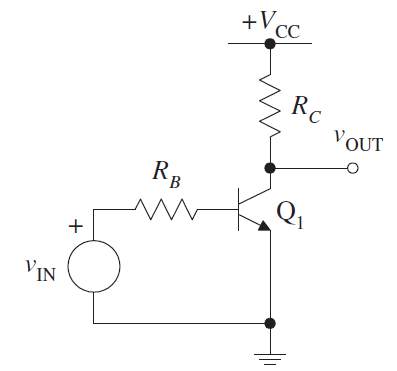
\includegraphics[width=\linewidth]{Schematic_Inverter.png}
    \caption{Schema circuitale}
  \end{subfigure}
  \hspace{0.05\textwidth}
  \begin{subfigure}{0.45\textwidth}
    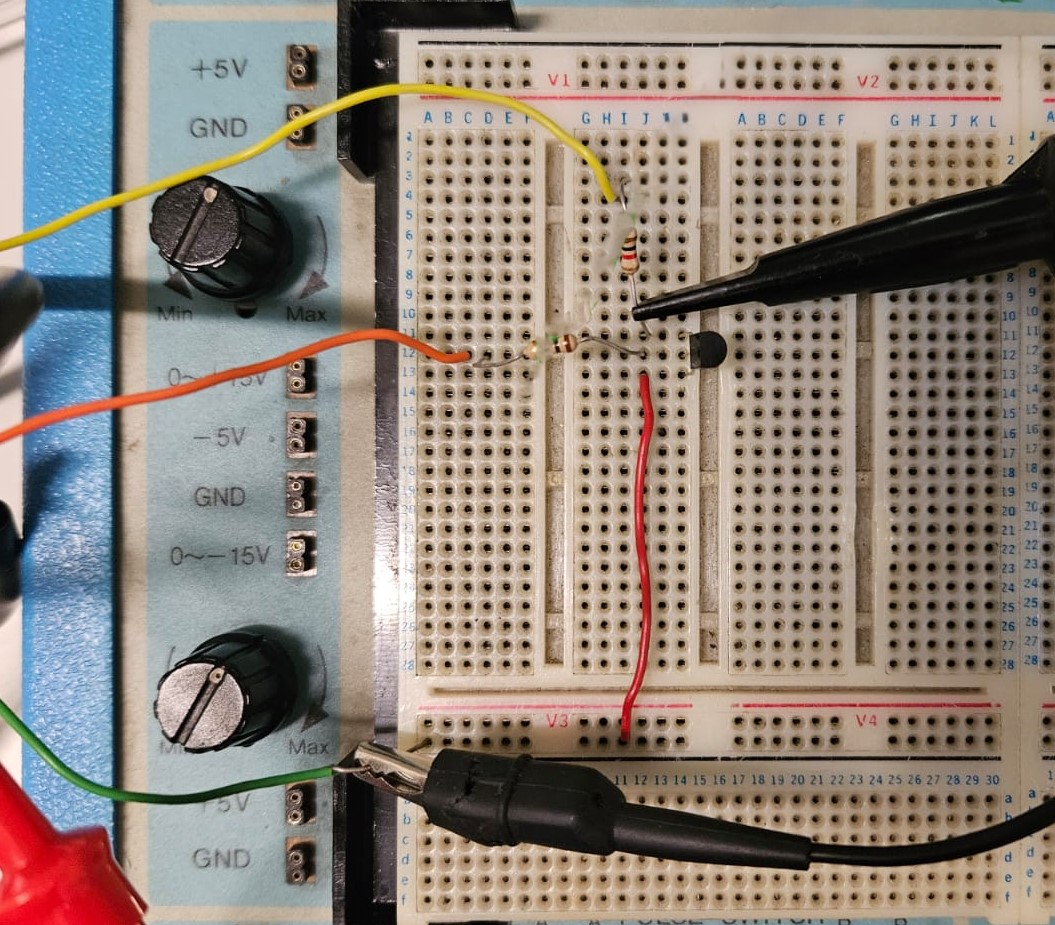
\includegraphics[width=\linewidth]{Inverter_montato.jpg}
    \caption{Circuito assemblato}
  \end{subfigure}
  \caption{Inverter RTL}
\end{figure}

Il circuito è costituito da resistenze dal valore di \(R_B = (\,0.990\,\pm\, 0.001 )\, k\Omega\) e di \(R_B = (\,0.990\,\pm\, 0.001 )\, k\Omega\) e da un Transistore Bipolare a Giunzione di tipo NPN del modello BC547C, la cui base \(v_{in}\) è alimentata da un segnale ad onda quadra da ampiezza \(V_{pp}^{in} = (\,5.000 \,\pm\, 0.001\,)\, V\) con un offset di correnta continua di \(V_{offset}^{in} = (\,5.000\, \pm \,0.001\,)\, V\) e frequnza \(f_{out}= (\,1.500\, \pm\, 0.001\, )\, kHz \), mentre il collettore è alimentato da una tensione costante \(V_{CC}=(\,5.000\, \pm\, 0.001\, )\, \mathrm{kHz} \).
Inizialmente ci siamo soffermati sull'analisi della forma d'onda osservata dalla sonda all'uscita \(v_{out}\). Come è possibile osservare dall'immagine \ref{fig onda_inverter}, fornendo l'onda del canale CH1 al terminale \(v_{in}\), il segnale di \(v_{out}\) segue il comportamento atteso. L'onda emessa dal circuito risulta infatti essere non altro che un'onda quadra invertita dalla frequenza \(f_{out}= (\,1.500\, \pm\, 0.001\, )\, kHz \), uguale a quella di ingresso, e dai valori \(V_{OH} = (\,5.0\, \pm\, 0.2\,)\,V\), con lo stesso offset di continua da \(V_{OL} = (\,0.0 \,\pm\,0.2\,)\,V\)\footnote{Le incertezze in questo caso sono state valutate l'ultima cifra siglificativa dei dati acquisiti con l'oscilloscopio }. 
\begin{figure}[ht]
  \centering
  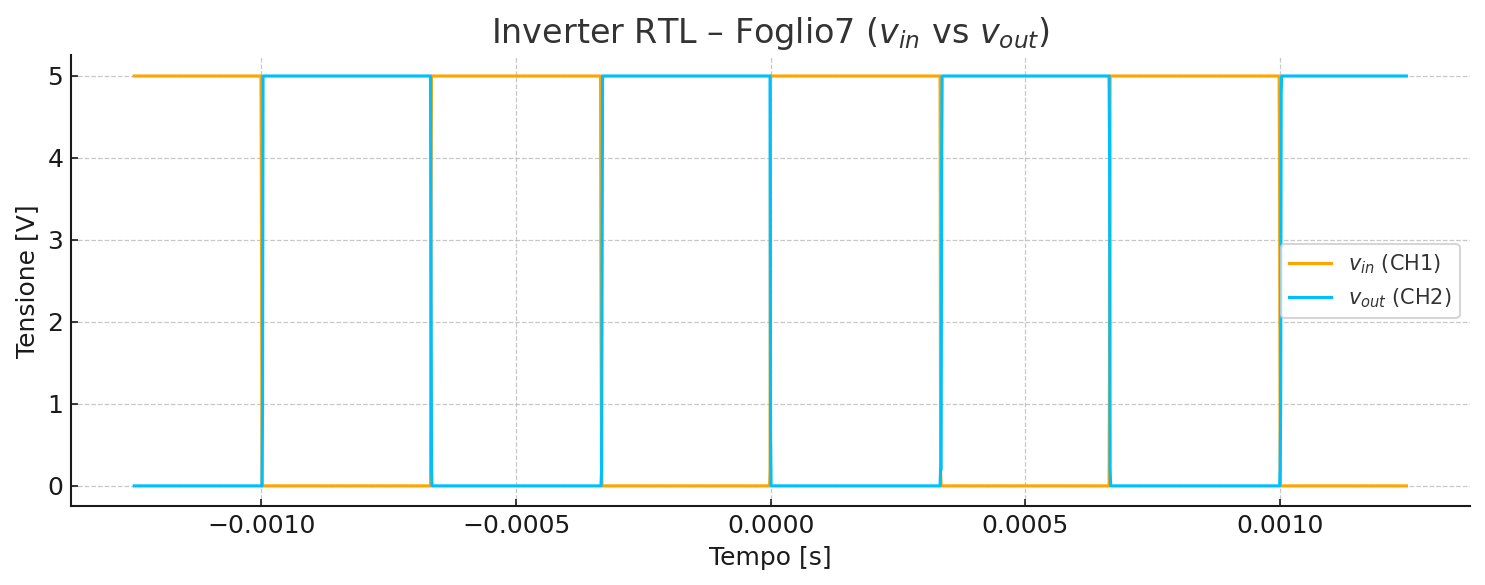
\includegraphics[width=0.9\textwidth]{onda_quadra.png}
  \caption{grafico di $v_{out}(t)$ (CH2) e di $v_{in}(t)$ (CH1), di un onda quadra}
  \label{fig:derivatore_sin}
\end{figure}

Dopo aver verificato il corretto funzionamento del circuito, ci siamo dedicati ad un'analisi più dettagliata dei segnali di una porta NOT in tecnologia RTL in salita e in discesa.

% \subsection{Analisi in discesa}
%   Come precedentemente annunciato, il comportamento del segnale \(v_{out}\) in fase di discesa, ossia quando il BJT si satura (tensione superiore a \(V_{\gamma} = \)), il collegamento tra l'emitter e il collector può essere considerato in prima approssimazione come un cortocircuito, allora la tesione misurata in \(v_{out}\) crolla perchè collegato alla terra.
%   Detto questo però si nota come il segnale non abbia caduta istantanea, ma la discesa viene pilotata dal transistore bipolare \(Q_1\) acceso, che funziona per un breve periodo come un generatore di corrente. La corrente trasmessa risulta essera la scarica della capacit`a di giunzione base-collettore del transistor che  viene scaricata a corrente elevata e costante.
% \begin{figure}[ht] \label{fig: discesa}
%   \centering
%   \begin{subfigure}{0.9\textwidth}
%     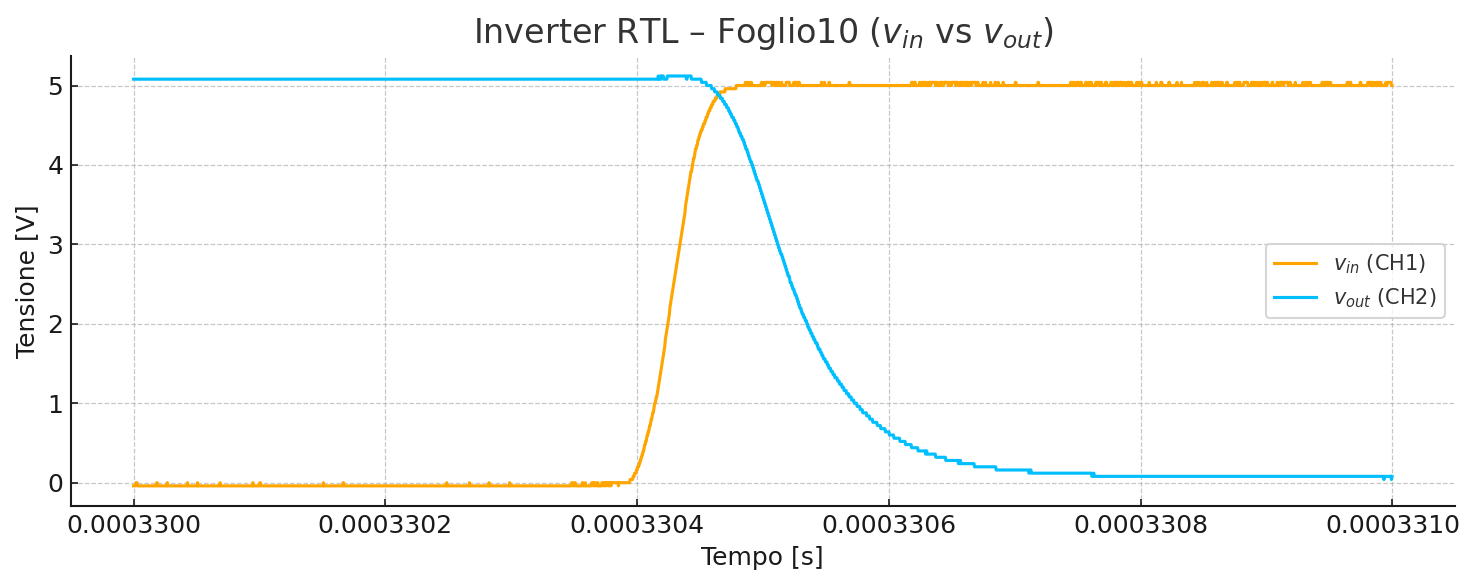
\includegraphics[width=\linewidth]{discesa.png}
%     \caption{grafico di $v_{out}(t)$ (CH2) e di $v_{in}(t)$ (CH1)}
%   \end{subfigure}
%   \hspace{0.05\textwidth}
%   \begin{subfigure}{0.9\textwidth}
%     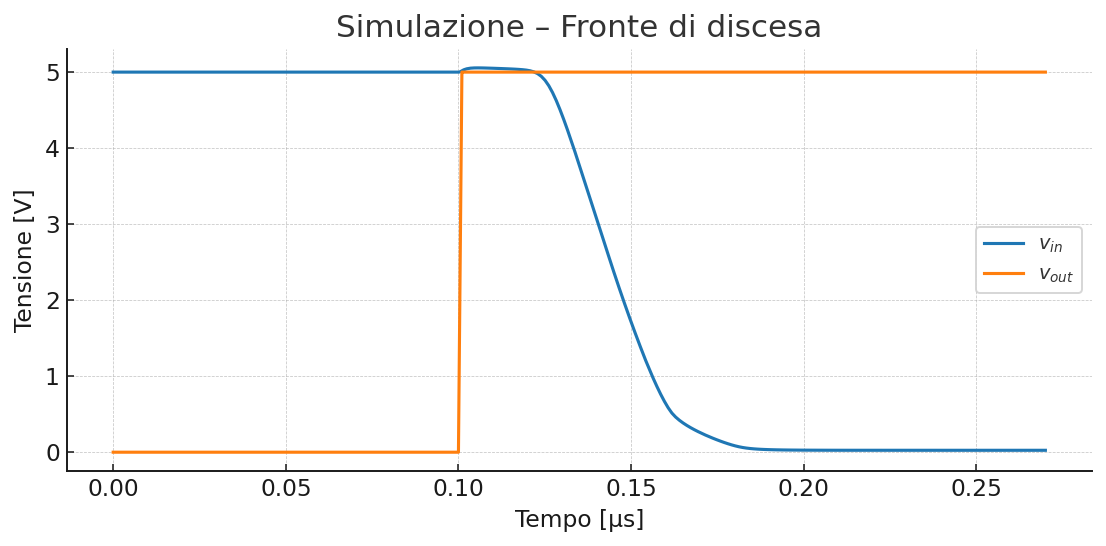
\includegraphics[width=\linewidth]{discesa_sim2.png}
%     \caption{Risultato simulazione}
%   \end{subfigure}
%   \caption{Inverter RTL}
% \end{figure}
% Come si può notare nella fugura \ref{fig: discesa} la discesa del segnale in uscita segue l'andamento atteso dalla simulazione. 

% Abbiamo poi misurato delle grandezze che descrivono l'andamento di segnale in discesa attraverso l'utilizzo della modalità cursori dell'oscilloscopio.
% Per prima cosa, abbiamo misurato il tempo di ritardo in discesa ottenendo \(t_{df}= 80 \ pm 10 ns\). Successivamente abbiamo ottenuto il tempo di discesa in uscita \(t_f = 80 \pm 10 ns\). Infine abbiamo misurato il valore della tensione di uscita al livello logico basso \(VOL = V_{CE,sat} = 40.8 \pm 0.1 mV\).
% Successivamente abbiamo misurato anche l'ampiezza dell'overshoot del segnale \(v_{out}\). In corrispondenza dell'accensione del transistore, ossia quando il segnale di \(v_{in}\) supera la soglia di saturazione, la tensione supera la tensione di alimentazione a causa della capacità di giunizione tra B-C quando il transistore è spento. Nel nostro caso l'Overshoot del segnale in uscita è risultato \(V_{os}= 60 \pm 20mV\). La misura risulta avere un errore relativo molto alto, questo è causa del fatto che l'Overshoot era significativamente più piccolo, e il cambio scala sull'oscillatore per la sua misura attraverso cursorei avrebbe implicato una perdita di trigger.
\subsection{Analisi in discesa}
Come precedentemente annunciato, il comportamento del segnale \(v_{out}\) in fase di discesa, ossia quando il BJT si satura (ovvero per tensioni di ingresso superiori a \(V_{\gamma} \approx 0.7\,\mathrm{V}\)), può essere modellato in prima approssimazione come un cortocircuito tra collettore ed emettitore. In questa condizione, la tensione misurata in \(v_{out}\) crolla poiché il collettore risulta connesso a massa.

Tuttavia, si osserva che la caduta non è istantanea. La discesa è infatti guidata dal transistore bipolare \(Q_1\), acceso, che per un breve intervallo si comporta come un generatore di corrente costante. La corrente erogata serve a scaricare la capacità di giunzione base-collettore del transistor, determinando così un fronte di discesa definito e non verticale.

\begin{figure}[H] \label{fig: discesa}
  \centering
  \begin{subfigure}{0.9\textwidth}
    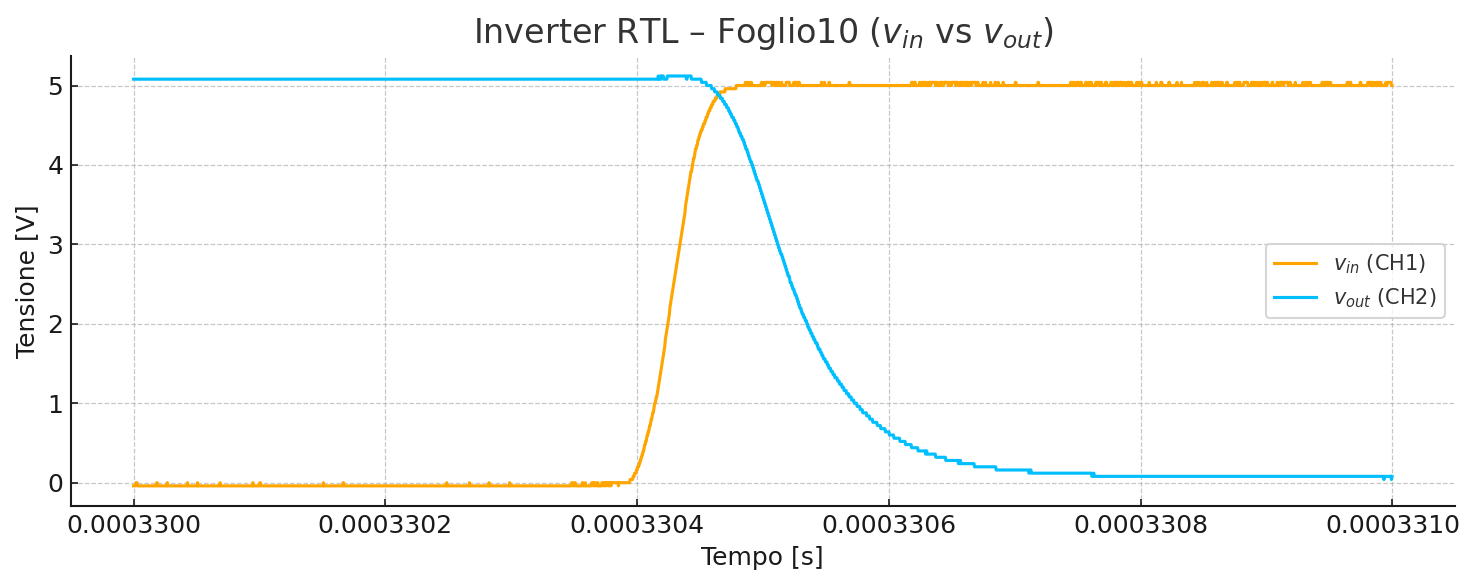
\includegraphics[width=\linewidth]{discesa.png}
    \caption{Grafico di \(v_{out}(t)\) (CH2) e di \(v_{in}(t)\) (CH1)}
  \end{subfigure}
  \hspace{0.05\textwidth}
  \begin{subfigure}{0.9\textwidth}
    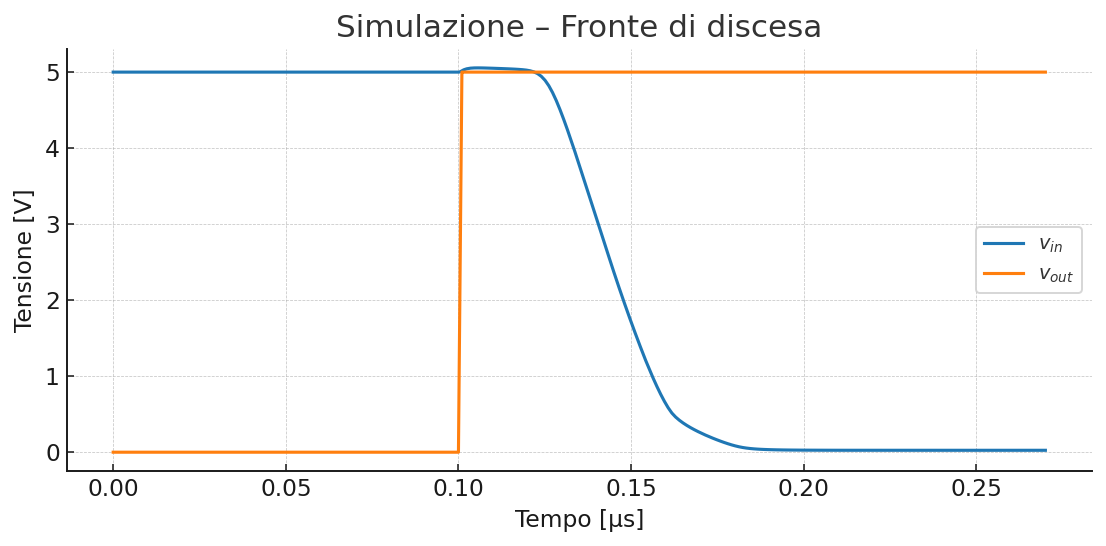
\includegraphics[width=\linewidth]{discesa_sim2.png}
    \caption{Risultato della simulazione LTspice}
  \end{subfigure}
  \caption{Fronte di discesa – Confronto tra misurazione sperimentale e simulazione}
\end{figure}

Come si può osservare nella figura \ref{fig: discesa}, la discesa del segnale in uscita sperimentale segue l’andamento previsto dalla simulazione.

Abbiamo quindi misurato alcune grandezze caratteristiche della fase di discesa tramite la modalità “Cursor” dell’oscilloscopio:

\begin{itemize}
  \item Tempo di ritardo in discesa: \(t_{\text{df}} = (80 \pm 10)\,\mathrm{ns}\)
  \item Tempo di discesa in uscita: \(t_{\text{f}} = (80 \pm 10)\,\mathrm{ns}\)
  \item Livello logico basso: \(V_{\text{OL}} = V_{\text{CE,sat}} = (41 \pm 4)\,\mathrm{mV}\)
\end{itemize}

Inoltre, è stata rilevata la presenza di un overshoot negativo del segnale \(v_{out}\), in corrispondenza dell'accensione del transistore (cioè nel momento in cui \(v_{in}\) supera \(V_\gamma \approx 0.7 V\) per il transistore BC547C). Ciò è dovuto alla rapida scarica della capacità di giunzione base-collettore, che genera un picco negativo temporaneo. L'ampiezza misurata dell'overshoot è risultata:
\[
V_{\text{OS}} = (60 \pm 20)\,\mathrm{mV}
\]

La relativa incertezza è significativa poiché l’ampiezza dell’overshoot è molto ridotta rispetto all’intervallo dinamico del segnale, il che comporta un aumento scala ulteriore, per una misura più precisa, sarebbe risultata in una perdiata del trigger del segnale.


% . Inoltre, per catturarlo è stato necessario rinunciare al trigger automatico, riducendo l'affidabilità della misura. Il cambio scala richiesto per osservarlo chiaramente ha comportato un aumento dell’incertezza nella lettura.

% La misura risulta avere un errore relativo molto alto, questo è causa del fatto che l'Overshoot era significativamente più piccolo rispetto al segnale, e il cambio scala sull'oscillatore per la sua misura attraverso cursorei avrebbe implicato una perdita di trigger.

% \subsection{Analisi in salita}
% Una analoga procedura è sata seguita per l'analisi del segnale \(v_{out}\) in salita, ossia quando il segnale \(v_{in}\) scende sotto la soglia di saturazione, polarizzando inversamente entrambe le giunzioni, rendendo il transistore equivale ad una coppia di diodi in polarizzazione inversa. Perciò Il transistore funziona in Interdizione, cio`e si comporta come un interruttore spento e non permette il passaggio di corrente, perciò il segnale trasmesso in \(v_{out}\) risulta essere \(V_{CC}\).
% L'andamento in salita del segnale anche in questo caso risulta rallentato, siccome parte della corrente va a caricare il condensatore di giunzione del transistore Q1 con una costante di tempo \(\tau = R_CC_{junc}\), dove \(C_{junc}\) è la capacità del condensatore di giunzione, collegato in parallelo al transistore Q1. 
% \begin{figure}[ht] \label{fig: salita}
%   \centering
%   \begin{subfigure}{.6\textwidth}
%     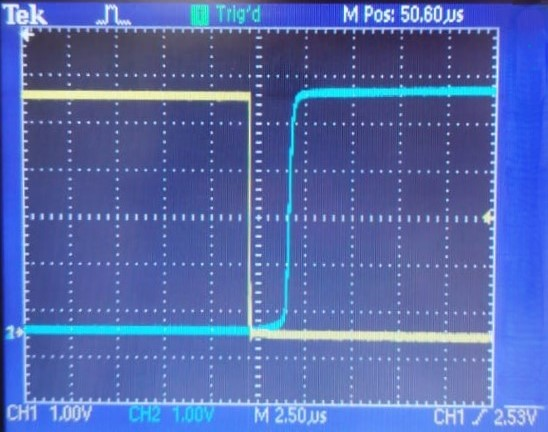
\includegraphics[width=\linewidth]{salita_def.jpg}
%     \caption{grafico di $v_{out}(t)$ (CH2) e di $v_{in}(t)$ (CH1)}
%   \end{subfigure}
%   \hspace{0.05\textwidth}
%   \begin{subfigure}{0.9\textwidth}
%     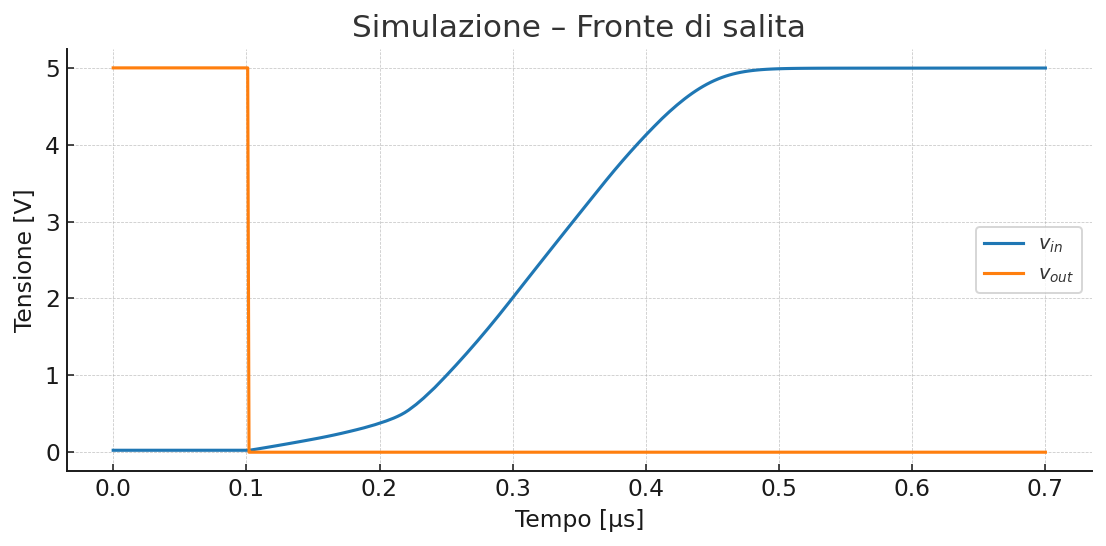
\includegraphics[width=\linewidth]{salita_sim2.png}
%     \caption{Risultato simulazione}
%   \end{subfigure}
%   \caption{Inverter RTL}
% \end{figure}

% Abbiamo poi misurato delle grandezze che descrivono l'andamento di segnale in salita attraverso l'utilizzo della modalità cursori dell'oscilloscopio.
% Per prima cosa, abbiamo misurato il tempo di ritardo in salita ottenendo \(t_{dr}= 2.10 \ pm  \mu s\). Successivamente abbiamo ottenuto il tempo di salita in uscita \(t_r = 420 \pm 10 ns\). Infine abbiamo misurato il valore della tensione di uscita al livello logico basso \(VOH = 40.8 \pm 0.1 mV\).
\subsection{Analisi in salita}
Una procedura analoga è stata seguita per l'analisi del segnale \(v_{out}\) in salita, ovvero quando il segnale \(v_{in}\) scende al di sotto della soglia di saturazione \(V_\gamma \approx 0.7\,\mathrm{V}\), polarizzando inversamente entrambe le giunzioni del BJT. In questa condizione, il transistore si trova in interdizione e si comporta come un interruttore aperto, impedendo il passaggio di corrente tra collettore ed emettitore. Di conseguenza, il nodo di uscita \(v_{out}\) risale verso la tensione di alimentazione \(V_{CC}\).

L’andamento del fronte di salita non è istantaneo, ma rallentato dalla presenza della capacità di giunzione collettore-base del transistore, che deve essere caricata tramite la resistenza di pull-up \(R_C\). La costante di tempo associata a questo processo è:
\[
\tau = R_C C_{\text{junc}}
\]
dove \(C_{\text{junc}}\) è la capacità parassita tra collettore e base del transistore \(Q_1\).

\begin{figure}[H] \label{fig: salita}
  \centering
  \begin{subfigure}{0.7\textwidth}
    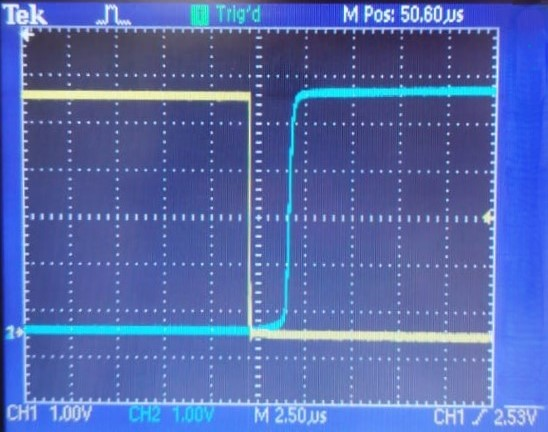
\includegraphics[width=\linewidth]{salita_def.jpg}
    \caption{Grafico di \(v_{out}(t)\) (CH2) e \(v_{in}(t)\) (CH1) – Oscilloscopio}
  \end{subfigure}
  \hspace{0.05\textwidth}
  \begin{subfigure}{0.9\textwidth}
    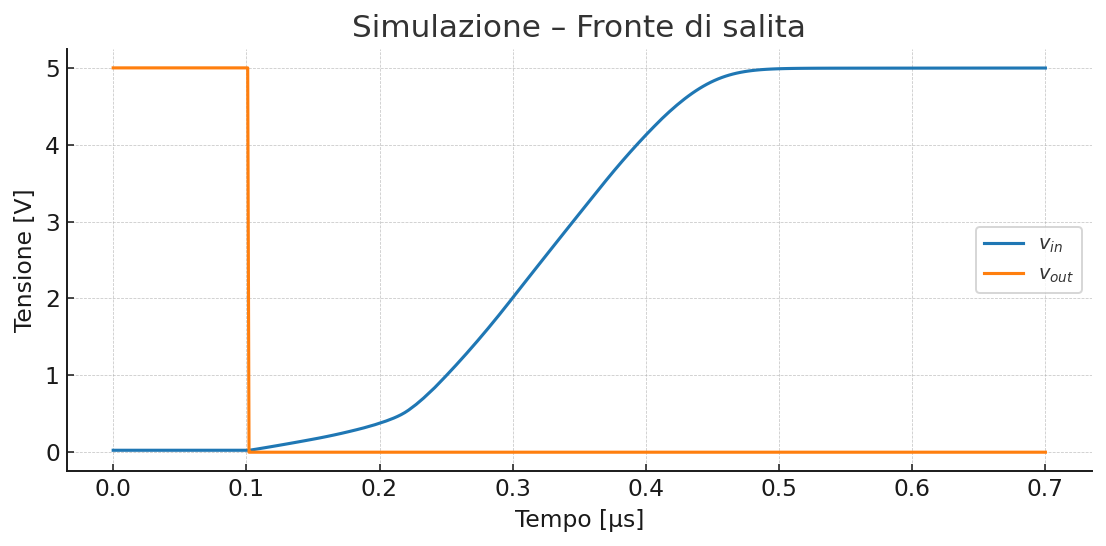
\includegraphics[width=\linewidth]{salita_sim2.png}
    \caption{Risultato della simulazione LTspice}
  \end{subfigure}
  \caption{Fronte di salita – Confronto tra misura sperimentale e simulazione}
\end{figure}

Come si osserva nella figura \ref{fig: salita}, il fronte di salita misurato presenta un andamento coerente con quello simulato: la tensione di uscita impiega un tempo finito per risalire al valore logico alto, mostrando un’evidente costante di tempo esponenziale.

Sono state misurate le seguenti grandezze, utilizzando la modalità “Cursor” dell’oscilloscopio:

\begin{itemize}
  \item Tempo di ritardo in salita: \(t_{\text{dr}} = (2.10 \pm 0.10)\,\mu\mathrm{s}\)
  \item Tempo di salita del fronte di uscita: \(t_{\text{r}} = (420 \pm 10)\,\mathrm{ns}\)
  \item Livello logico alto: \(V_{\text{OH}} = (5.000 \pm 0.004)\,\mathrm{V}\)
\end{itemize}

Tutti i valori sono risultati compatibili con il comportamento atteso del circuito Inverter RTL in fase di risalita, tenendo conto dei tempi di carica imposti dalla rete resistivo-capacitiva del nodo di uscita.


% \subsection{Analisi della Caratteristica Statica}
% Successivamente abbiamo studiato sia la caratteristica statica del circuito descritto dalla \ref{fig: inverter} e dell'analogo ma dal transistore BC547C invertendo la sua orientazione.
% Innanzitutto abbaimo impostato un segnale di onda triangolare di frequenza \(f_{in} = 500 \pm Hz\), di ampiezza \(V_{in,A} = 5.08 \pm V\), offeset di corrente continua di \(V_{offset} = 5V\), con parametro di simmetria impostato a \(50\%\) e una \(V_{CC} = 5V\).

% \begin{figure}[ht]
%   \centering
%   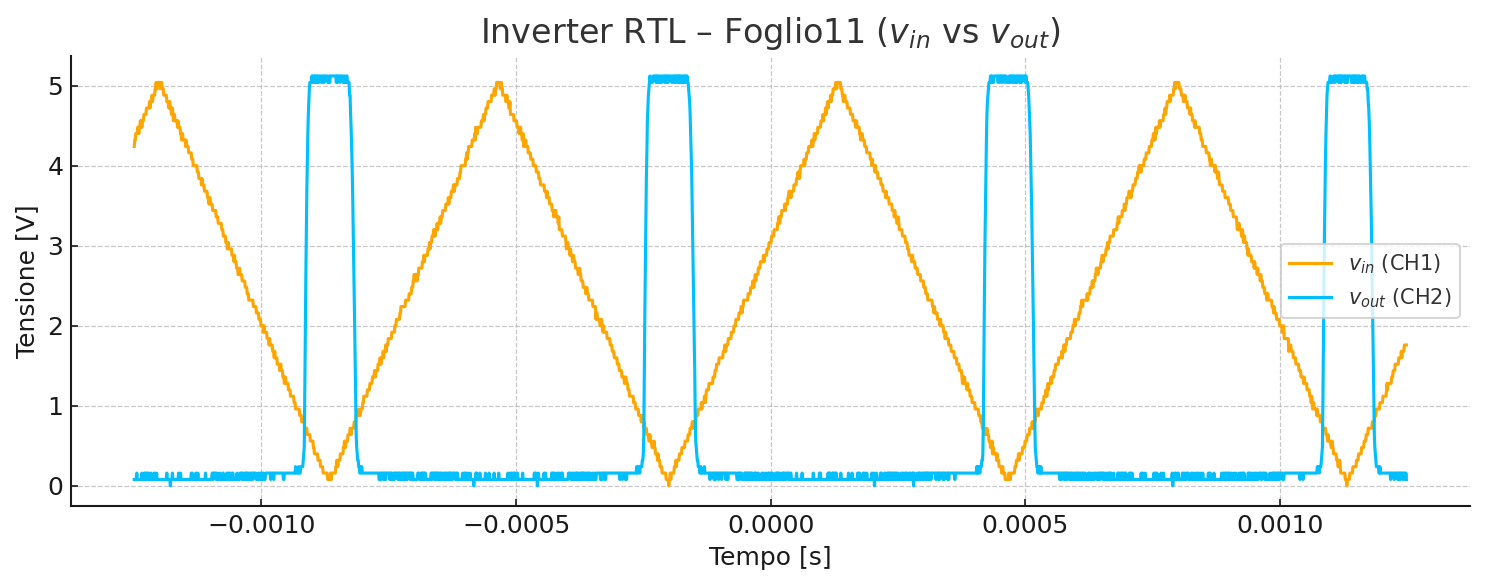
\includegraphics[width=0.9\textwidth]{triangolare2.png}
%   \caption{grafico di $v_{out}(t)$ e di $v_{in}(t)$, di un onda sinosuidale}
%   \label{fig:derivatore_sin}
% \end{figure}


% Il segnale \(v_{out}\) ottenuto, risulta quello atteso: delle pulsazioni periodiche della stessa frequenza \(f_{in}\) ma di un periodo di attivazione di \(t_{on} = 3.0 \pm 1.0 \mu s \), che conincide con la parte di segnale di ingresso che sta sotto la soglia di saturaizione ... 
% Successivamente abbiamo impostato la modalità di visualizzazione dell'oscilloscopio a XY, permettendoci di osservare la Caratteristica Statica del sistema \(v_{out}-v{in}\), mostrando perciò sull'asse delle X il segnale proveniente dal canale \(CH1\), ossia \(v_{in}\), e sull'asse delle Y il segnale di \(CH2\), ossia \(v_{out}\). 
% Come è possibile osservare dall'immagine \ref{fig: } si nota che subito come il comportamento del sistema coincida con quello atteso.

% \begin{figure}[ht] \label{fig: caratteristica}
%   \centering
%   \begin{subfigure}{0.45\textwidth}
%     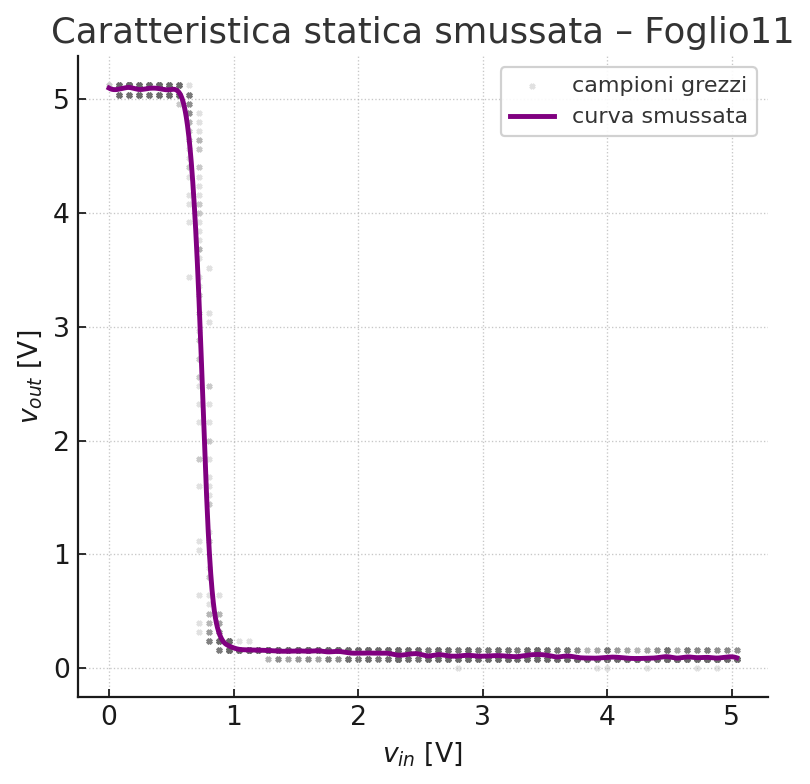
\includegraphics[width=\linewidth]{caratteristica_statica.png}
%     \caption{grafico di $v_{out}(t)$ (CH2) e di $v_{in}(t)$ (CH1)}
%   \end{subfigure}
%   \hspace{0.05\textwidth}
%   \begin{subfigure}{0.45\textwidth}
%     % \includegraphics[width=\linewidth]{}
%     \caption{Simulazione in LtSpice}
%   \end{subfigure}
%   \caption{Inverter RTL} \footnote{Il grafico della caratteristica statica risulta quello di una curva ottenute con un algoritmo di smoothing di media mobile valutata su 10 punti}
% \end{figure} 

% La forma tipica della caratteristica statica ingresso-uscita della porta NOT RTL è da attirbuire al modo in cui li segnale \(v_{out}\) si comporta relativamente al valore di tensione del segnale \(v_{in}\).
% Notiamo infatti che, quando il segnale \(v_{in}\) assume valori sotto la soglia di saturazione \(v_{\gamma} = 0.7V\), il segnale \(v_{out}\) assume il valore di \(V_{out, on} = 5.08 \pm V\). Quando il segnale \(v_{in}\) supera la soglia di \(V_\gamma = 0.7V\), il transistore comincia a far condurre corrente, collegando alla terra il terminale \(v_{out}\), il che riduce drasticamente il valore della tensione, la cui caduta è descritta dal gradino nel grafico.
% Al crescere del segnale del segnale \(v_{in}\) oltre \(V_\gamma\), il valore di \(v_{out}\) rimane constante e uguale a \(V_{out, off} = 0 \pm  V\), il che si traduce nella caratteristica statica del sistema in una retta orizzontale, fino a quando non il segnale \(v_{in}\) non raggionge il suo valor massimo di \(V_{in,max} = 5 \pm V\), per eseguire lo stesso percorso in maniera inversa. 
% Mentre negli scorsi paragrafi si è discusso il comportamento differente del segnale s'uscita in fase di  \textit{rise} e di \textit{fall}, argomentando sul come il comportamento del sistema è perciò asimmetrico, il grafico della Caratteristica Statica mostrato nell'immagine \ref{fig: caratteristica}, suggerirebbe invece che il percorso sia perfettamente simmetrico. Questo perchè il grafico mostra una linea curva aperta invece di un percorso chiuso. \footnote{Un percorso chiuso aperto indica che, relativamente al valore del segnale d'ingresso, quello di uscita assume gli stessi valori a prescindere della direzione in cui sta percorrendo il segnale d'ingresso. Mentre una curva chiusa distinta indica, si che il segnale è periodico e continuo, ma che non è simmetrico rispetto alla direzione id \(v_{in}\) } 
% Questa osservazione è cade però nel momento in cui si va a zoomare orizzontalmente e verticalmete il diagramma a XY, osserviamo che il segnale di uscita segeue in realtà due traiettorie differenti se in fase di \textit{rise} e di \textit{fall}, confermando quel che abbiamo osservato precedentemente.
% Trascurando questo comportamento, ci siamo concentrati nella misura del guadagno \(\beta\) attraverso la stima del coefficiente angolare della retta che descrive l'andamento in \textit{rise} e \textit{fall} nel diagramma della Caratteristica Statica, ottenendo la misura di \(\beta = 220.85 \pm \) il che risulta compatibile con il valore atteso \dots di \dots.
% La incertezza cosniderata per questa misurazione sono un quadratino della griglia in relazione alla scala utilizzata per la misura.
% \begin{figure}[ht] \label{fig: caratteristica}
%   \centering
%   \begin{subfigure}{0.45\textwidth}
%     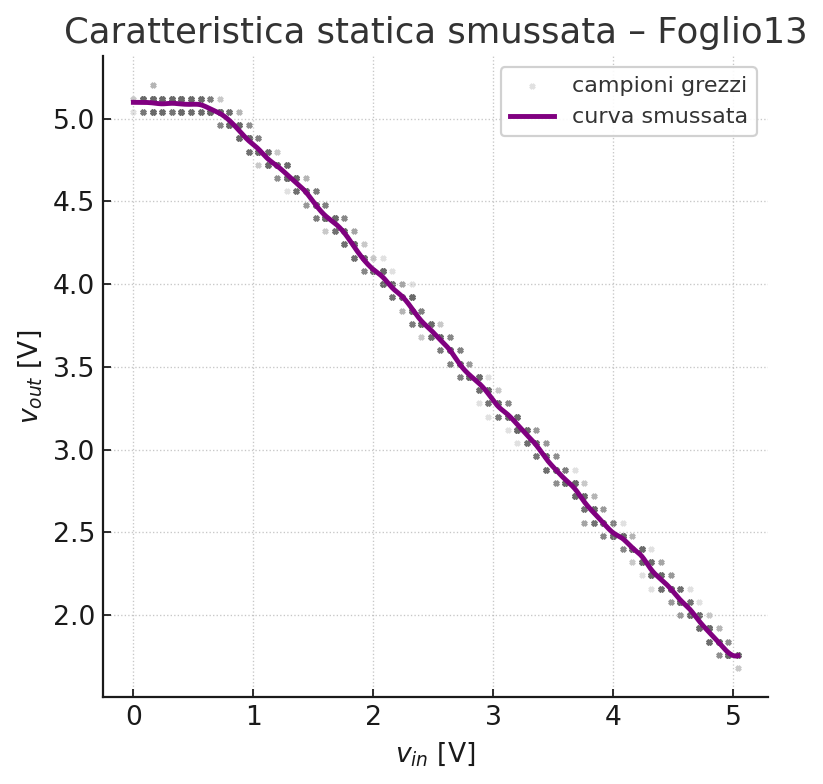
\includegraphics[width=\linewidth]{caratteristica_inver.png}
%     \caption{grafico della Caratteristica Statica di $v_{out}(t)$ (CH2) e di $v_{in}(t)$ (CH1)}
%   \end{subfigure}
%   \hspace{0.05\textwidth}
%   \begin{subfigure}{0.45\textwidth}
%     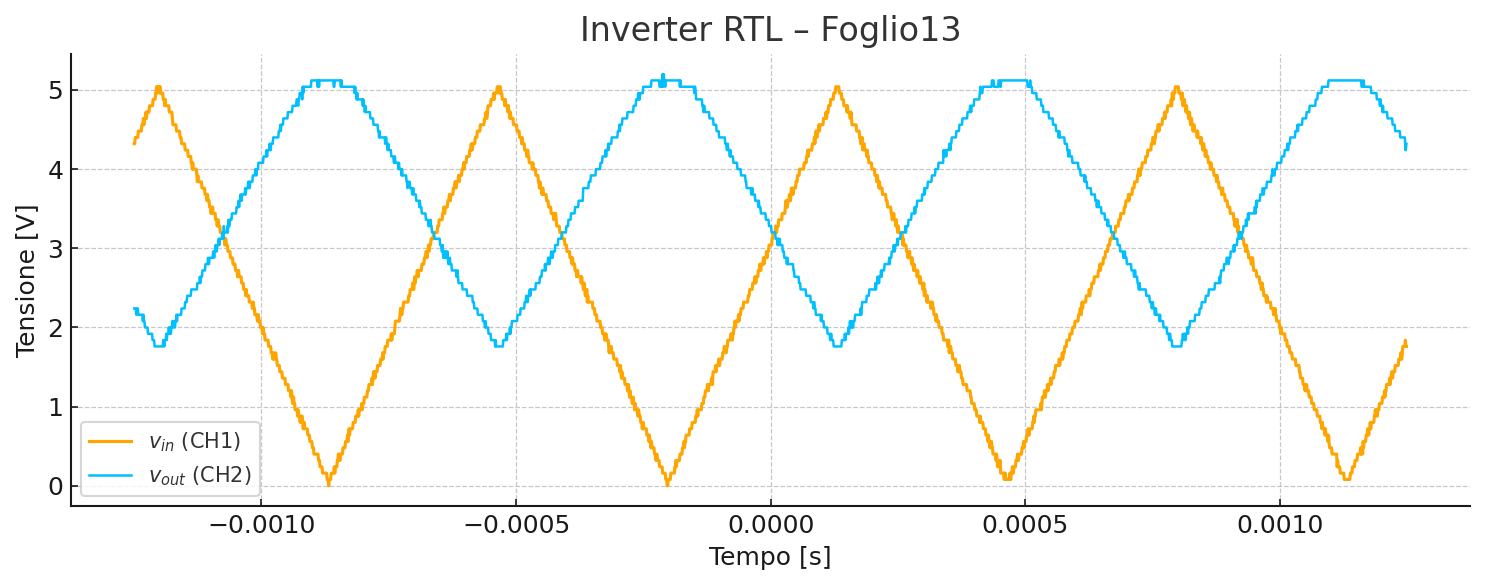
\includegraphics[width=\linewidth]{Triangolare_inver.png}
%     \caption{}
%   \end{subfigure}
%   \caption{}\footnote{Il grafico della caratteristica statica risulta quello di una curva ottenute con un algoritmo di smoothing di media mobile valutata su 10 punti}
% \end{figure}
% Successivamente abbiamo ripetuto questa procedura, ma invertendo la orientazione del transistore bipolare a giunzione per poi osservare il suo comportamento in questa configurazione e ripetere la misurazione di \(\beta\).
% Come mostrato nell'immagine \ref{fig: caratteristica_invertita} si può vedere come si comporta il circuito nel dominio del tempo... Perchè????
% Abbiamo successivamente misurato nuovamente il guadagno \(\beta_{inv}\) in maniera analoga, ottenendo \(\beta_{inv} = 8.76 \pm \), il che risulta compatibile con il valore atteso.


\subsection{Analisi della Caratteristica Statica}

Successivamente, abbiamo studiato la caratteristica statica del circuito Inverter RTL riportato in figura \ref{fig: inverter}, nonché quella del medesimo circuito con il transistore BC547C orientato in maniera invertita.

Per entrambe le configurazioni, è stato applicato un segnale triangolare al terminale di ingresso \(v_{in}\), con le seguenti caratteristiche:
\[
f_{in} = (1.500 \pm 0.006)\,\mathrm{kHz}, \quad V_{pp}^{in} = (5.000 \pm 0.004)\,\mathrm{V}, \quad V_{\text{offset}} = (5.000 \pm 0.004)\,\mathrm{V}
\]
La simmetria del segnale è stata impostata al \(50\%\) e l’alimentazione fornita al collettore era \(V_{CC} = (5.00 \pm 0.01)\,\mathrm{V}\).

\begin{figure}[H]
  \centering
  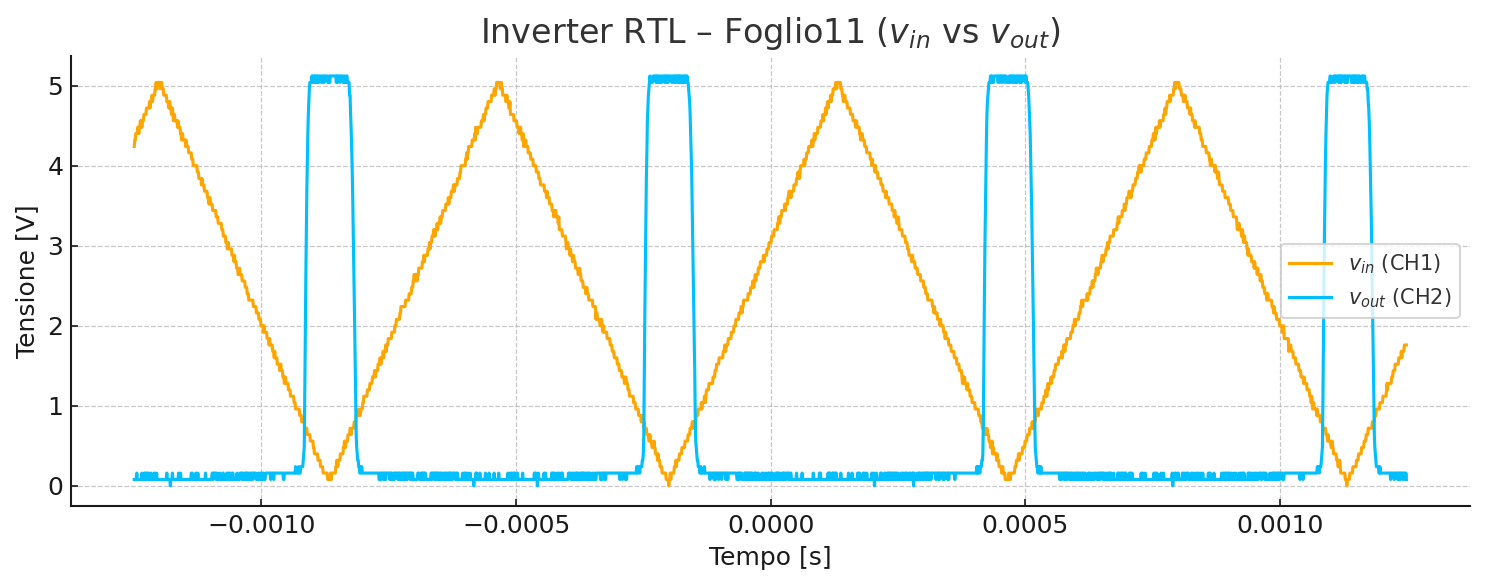
\includegraphics[width=0.9\textwidth]{triangolare2.png}
  \caption{Segnali \(v_{in}(t)\) (CH1) e \(v_{out}(t)\) (CH2) – Inverter RTL in configurazione standard}
  \label{fig: inverter-triangolare}
\end{figure}

Nel caso standard, il segnale \(v_{out}\) si comporta come atteso: si osservano impulsi rettangolari sincronizzati con la porzione di \(v_{in}\) che rimane sotto la soglia di conduzione \(V_\gamma\). Il tempo di attivazione misurato è \(t_{\text{on}} = (3.0 \pm 0.1)\,\mu\mathrm{s}\).

Successivamente, è stata attivata la modalità \texttt{XY} sull’oscilloscopio, per osservare graficamente la relazione statica tra \(v_{in}\) e \(v_{out}\). Il risultato, mostrato in figura \ref{fig: caratteristica_rtl}, è una curva non lineare che presenta un punto di transizione netto attorno a \(V_{\gamma} \approx 0.7\,\mathrm{V}\).

\begin{figure}[H] \label{fig: caratteristica_rtl}
  \centering
  \begin{subfigure}{0.45\textwidth}
    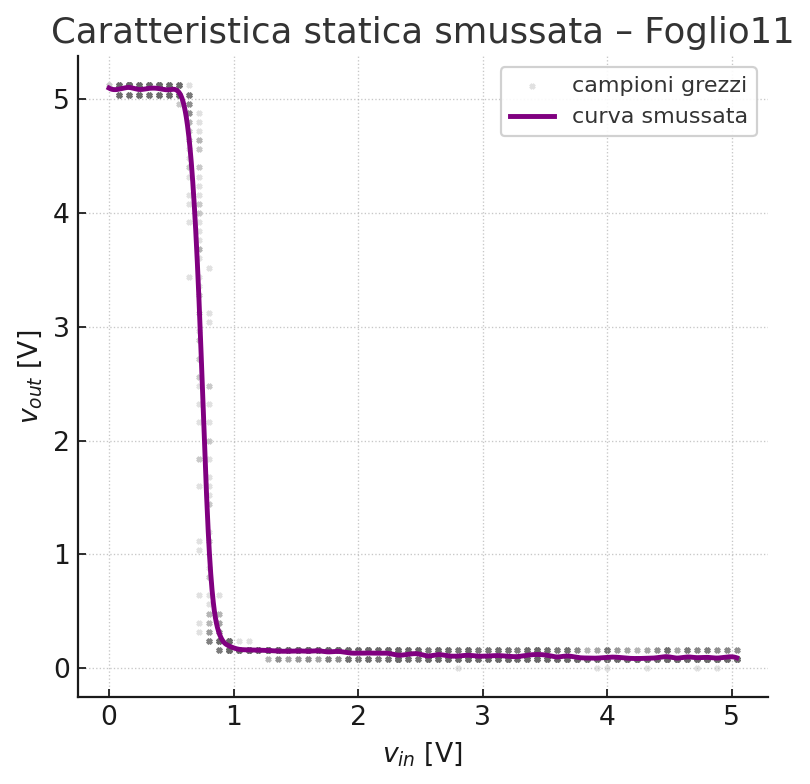
\includegraphics[width=\linewidth]{caratteristica_statica.png}
    \caption{Caratteristica statica (BC547C, orientazione standard)}
  \end{subfigure}
  \hfill
  \begin{subfigure}{0.45\textwidth}
    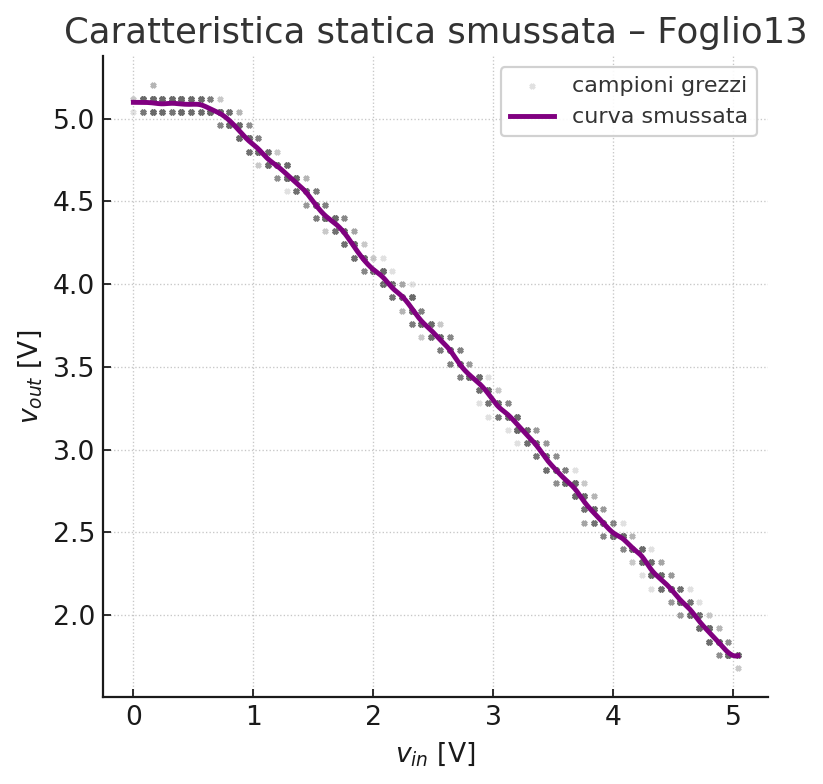
\includegraphics[width=\linewidth]{caratteristica_inver.png}
    \caption{Caratteristica statica (BC547C, orientazione invertita)}
  \end{subfigure}
  \caption{Curve caratteristiche statiche ottenute mediante visualizzazione XY. I punti grezzi sono stati smussati tramite media mobile su 10 punti.}
\end{figure}

Nel primo caso (orientazione standard), si osserva una caduta netta della tensione di uscita \(v_{out}\) non appena \(v_{in}\) supera \(V_\gamma\), coerente con la saturazione del transistor. La tensione d’uscita passa dal valore $V_{OH}$ a $V_{OL}$, precedentemente misurati.

Nel secondo caso (orientazione invertita), invece, la curva risulta molto più morbida e presenta un andamento quasi lineare decrescente. Questo è dovuto al fatto che il transistor, orientato in modo scorretto, non entra correttamente né in interdizione né in saturazione, ma opera in una regione intermedia non ben definita.

\begin{figure}[H]
  \centering
  \begin{subfigure}{0.9\textwidth}
    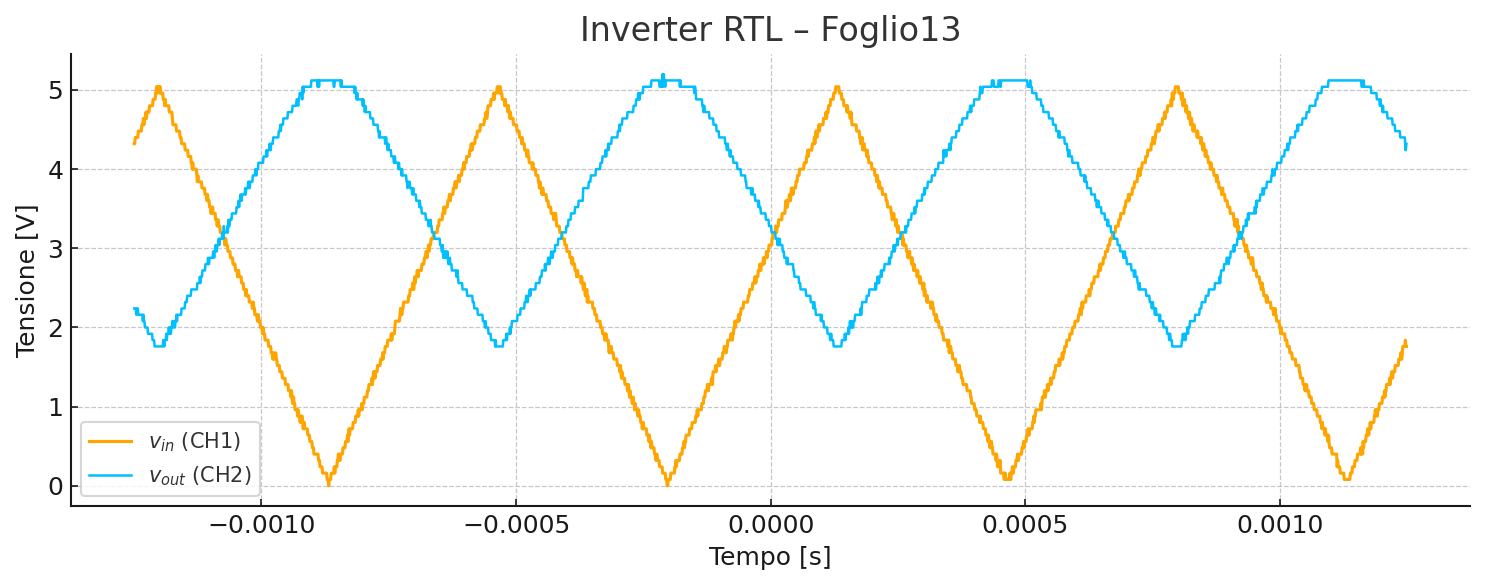
\includegraphics[width=\linewidth]{Triangolare_inver.png}
    \caption{Andamento nel dominio del tempo – transistor invertito}
  \end{subfigure}
  \caption{Risposta del circuito nel dominio del tempo con transistor invertito (BC547C). Si noti la forma non completamente logica dell’uscita.}
  \label{fig: inverter-invertito}
\end{figure}

Dal confronto tra le due configurazioni è stato possibile stimare il guadagno in corrente \(\beta\) del transistor in entrambe le situazioni attraverso la relazione \ref{eq: guadagno}, a partire dalla pendenza della curva nella regione di transizione. Si è ottenuto:
\[
\beta_{\text{standard}} = (221 \pm 8), \quad \beta_{\text{inverso}} = (8.76 \pm 0.08)
\]

Tali valori sono compatibili con quelli attesi: nel primo caso, \(\beta\) è elevato e coerente con le specifiche del BC547C, mentre nel secondo, l’inversione dei terminali degrada fortemente le capacità di amplificazione del dispositivo.

Inoltre, un’osservazione dettagliata del grafico XY mostra che, sebbene la curva sembri simmetrica, essa presenta due traiettorie distinte durante i fronti di salita e discesa, confermando il comportamento asimmetrico discusso nei paragrafi precedenti. Lo scostamento tra i due rami è dovuto alla diversa dinamica di carica/scarica della capacità di giunzione.

\medskip

Infine, riportiamo la nota che le curve mostrate sono state ottenute mediante un algoritmo di smoothing basato su media mobile di finestra pari a 10 campioni per rendere più leggibile la transizione statica.



% \subsection{Porta NOR RTL}
% Il secondo circuito assemblato e analizzato è quello di una porta logica NOR RTL secondo la schematica riportata nell'immagine \ref{fig: inverter}.

% \begin{figure}[ht] \label{fig: inverter}
%   \centering
%   \begin{subfigure}{0.45\textwidth}
%     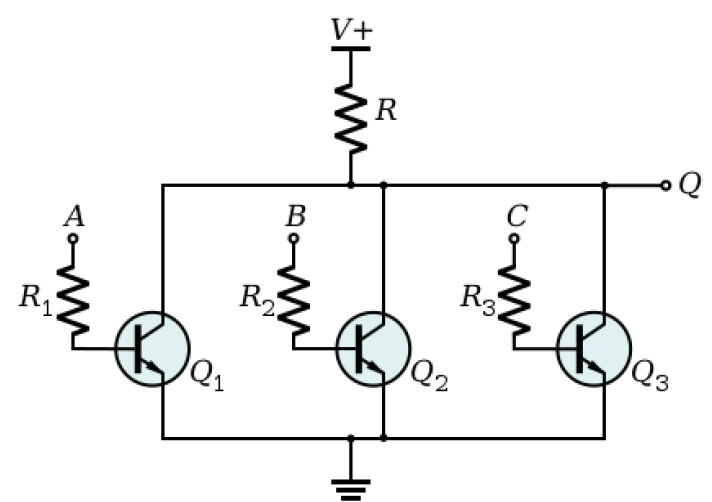
\includegraphics[width=\linewidth]{schema_NOR.png}
%     \caption{Schema circuitale}
%   \end{subfigure}
%   \hspace{0.05\textwidth}
%   \begin{subfigure}{0.45\textwidth}
%     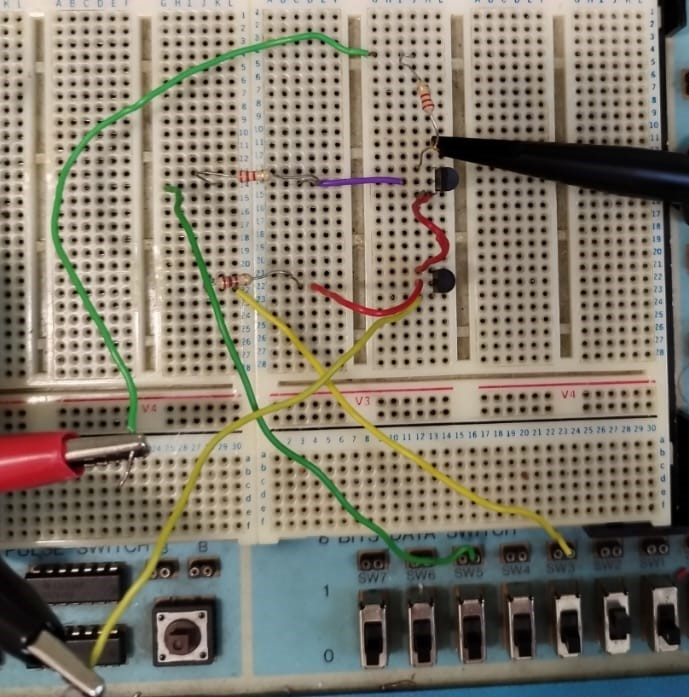
\includegraphics[width=\linewidth]{NOR2.jpg}
%     \caption{Circuito assemblato}
%   \end{subfigure}
%   \caption{Inverter RTL}
% \end{figure}

% Il circuito è costituito da una restistenza \textit{pull-up} dal valore di \(R = 9.903\pm 0.001 k\Omega\) e una \textit{pull-down} costituita da 3 transistori bipolare di giunizione NPN di modello BC547C, le cui basi collegate a una resistenza da \(R_{1,2,3} = 2200\pm 0.001 k\Omega\).
% Lo studio di questo circuito, in qualità di porta logica, è consistito nella verifica del comportamento atteso rispetto al comportamento atteso.
% Abbiamo alimentato gli switches incorporati con il banco e abbiamo così accesi e spenti per la verifica del funzionamento.
% (Spiega come mai funziona: anche se solo uno è attivo allora si spegne etc)
%  Come mostrato nella tabella delle misure 
% ... tabella
% Cè piena corrispondenza con quella attesa \ref{...}.

% \begin{figure}[ht] \label{fig: inverter}
%   \centering
%   \begin{subfigure}{0.45\textwidth}
%     \includegraphics[width=\linewidth]{.png}
%     \caption{Misurazione segnale 1}
%   \end{subfigure}
%   \hspace{0.05\textwidth}
%   \begin{subfigure}{0.45\textwidth}
%     \includegraphics[width=\linewidth]{.jpg}
%     \caption{Misurazione segnale 0}
%   \end{subfigure}
%   \caption{Inverter RTL}
% \end{figure}

% e alimentate da un segnale ad onda quadrata \(v_{in}\) da ampiezza \(V_{in,A} = 5.20 \pm 0.01\) con un offset di correnta continua di \(V_{offset} = 5.20 \pm 0.01 V\) e frequnza \(f_{in}= 1.000 \pm 0.001 Hz\), mentre il collettore è alimentato da una tensione costante \(V_{CC} = 5.00 \pm 0.01 V\).
% Inizialmente ci siamo soffermati sull'analisi della forma d'onda osservata dalla sonda all'uscita \(v_{out}\). Come è possibile osservare dall'immagine \ref{fig onda_inverter}, fornendo l'onda del canale CH1 al terminale \(v_{in}\), il segnale di \(v_{out}\) segue il comportamento atteso. L'onda emessa dal circuito risulta infatti essere non altro che un'onda quadra invertita dalla frequenza \(f_{out}= (1.000 \pm 0.001 )kHz \) e dall'ampiezza di \(V_{out} = 5.20 \pm 0.01V\), con lo stesso offset di continua da \(V_{offset} = 5.20 \pm 0.01V\). 



\subsection{Porta NOR RTL}

Il secondo circuito assemblato e analizzato è una porta logica NOR RTL, secondo la schematica riportata in figura \ref{fig: nor_schematics}.

\begin{figure}[H] \label{fig: nor_schematics}
  \centering
  \begin{subfigure}{0.45\textwidth}
    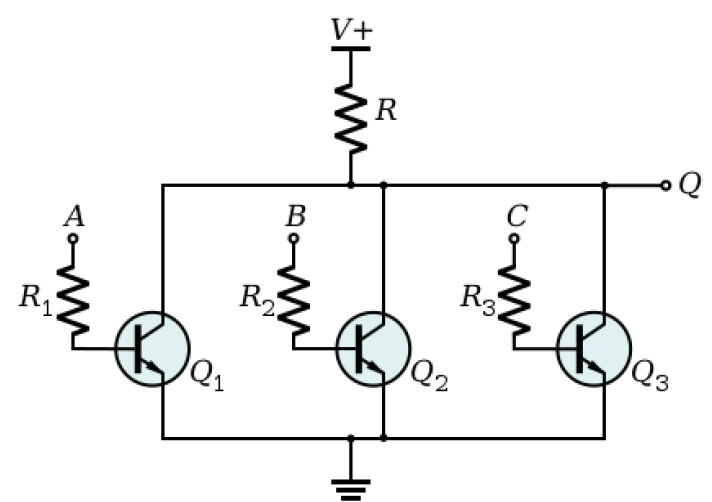
\includegraphics[width=\linewidth]{schema_NOR.png}
    \caption{Schema circuitale}
  \end{subfigure}
  \hfill
  \begin{subfigure}{0.45\textwidth}
    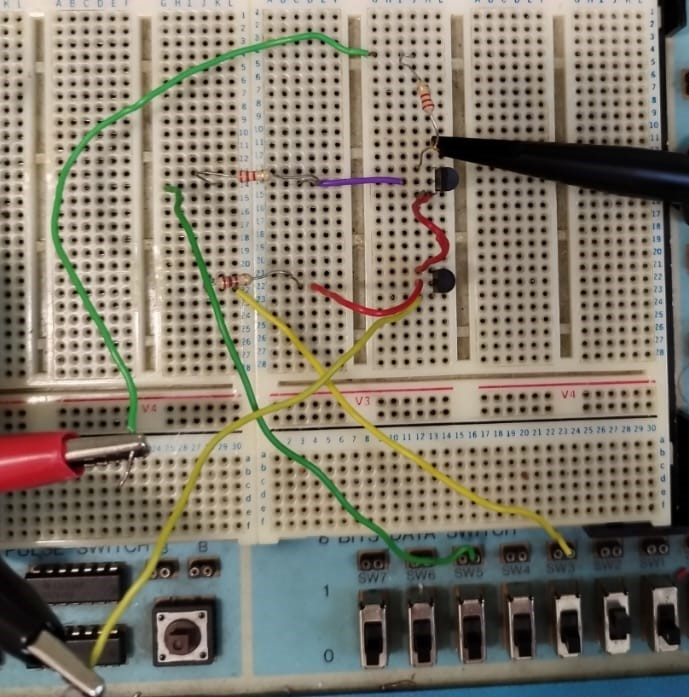
\includegraphics[width=\linewidth]{NOR2.jpg}
    \caption{Circuito montato su breadboard}
  \end{subfigure}
  \caption{Porta logica NOR RTL}
\end{figure}

Il circuito è costituito da: una resistenza \textit{pull-up} di valore \(R = (9.903 \pm 0.001)\,\text{k}\Omega\), tre transistori NPN (modello BC547C), collegati in parallelo come pull-down
e resistenze di base \(R_{1,2,3} = (2.200 \pm 0.001)\,\text{k}\Omega\).

Ogni base è connessa a un ingresso logico tramite uno degli interruttori del banco. Abbiamo alimentato il circuito con una tensione \(V_{CC} = (\,5\,\pm\,0.1\,)\,\mathrm{V}\) e testato le combinazioni logiche possibili degli ingressi attivando o disattivando gli switch.

Il comportamento osservato è perfettamente coerente con la tabella della verità teorica. In particolare:
\begin{itemize}
  \item se tutti gli interruttori sono aperti (ingressi a livello logico basso), nessun transistore conduce e il nodo di uscita si trova a livello alto: \(v_{out} = V_{CC}\)
  \item se anche uno solo degli ingressi è chiuso (livello logico alto), almeno un transistore satura e cortocircuita l'uscita verso massa: \(v_{out} \approx 0\,\mathrm{V}\)  
\end{itemize}

La seguente figura mostra l’uscita \(v_{out}\) osservata tramite oscilloscopio:

\begin{figure}[H] 
  \centering
  \begin{subfigure}{0.45\textwidth}
    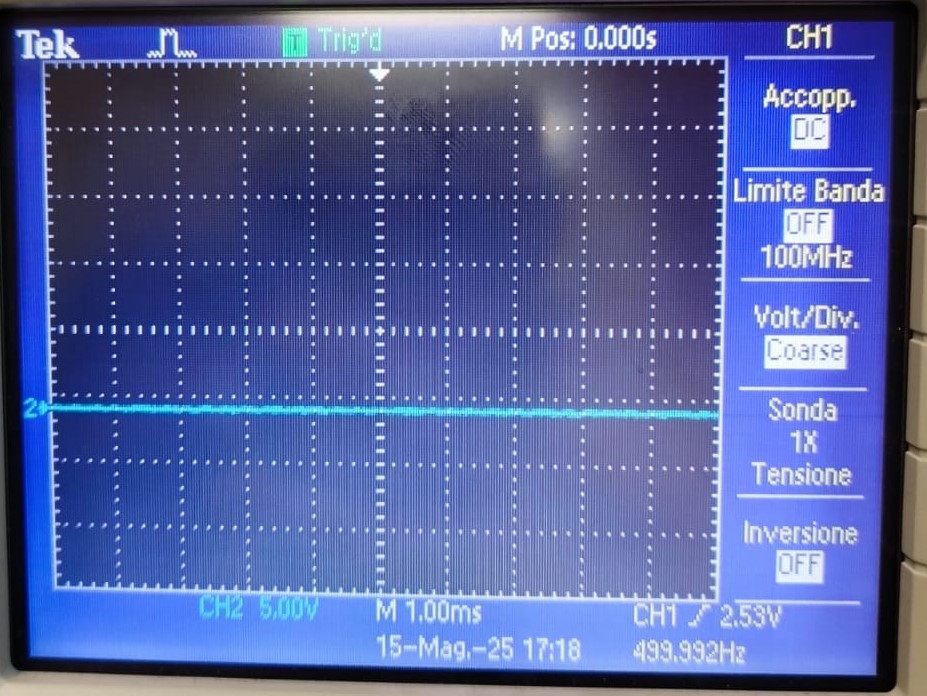
\includegraphics[width=\linewidth]{0.jpg}
    \caption{Uscita \(v_{out}(t)\) della porta NOR RTL in configurazione 0}
  \end{subfigure}
  \hfill
  \begin{subfigure}{0.45\textwidth}
    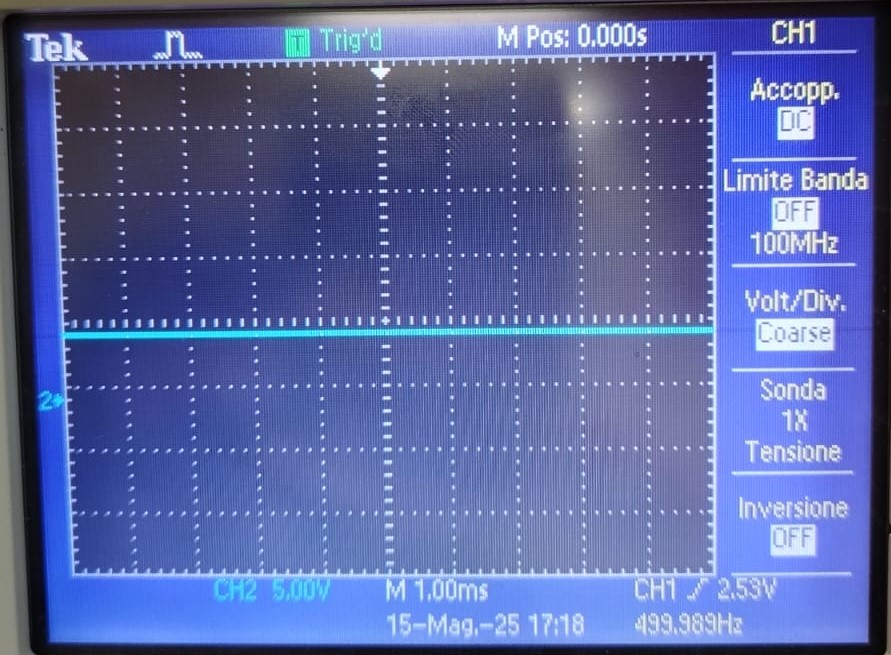
\includegraphics[width=\linewidth]{1.jpg}
    \caption{Uscita \(v_{out}(t)\) della porta NOR RTL in configurazione 1}
  \end{subfigure}
  \caption{Misura segnale porta logica NOR RTL}
\end{figure}

L’esperimento ha confermato il comportamento previsto: la porta NOR funziona correttamente e implementa l’operazione logica \(\overline{A + B + C}\). Ogni transistore agisce come uno "switch" verso massa: quando è attivo, forza il nodo di uscita a livello basso.

Il comportamento misurato è pienamente compatibile con la logica RTL NOR ideale, come riassunto nella tabella del parragrafo \ref{verita}.

\begin{table}[H] \label{tab:verita}
  \centering
  \begin{tabular}{ccc|c}
    A & B & C & \(Y = \overline{A + B + C}\) \\
    \hline
    0 & 0 & 0 & 1 \\
    0 & 0 & 1 & 0 \\
    0 & 1 & 0 & 0 \\
    0 & 1 & 1 & 0 \\
    1 & 0 & 0 & 0 \\
    1 & 0 & 1 & 0 \\
    1 & 1 & 0 & 0 \\
    1 & 1 & 1 & 0 \\
  \end{tabular}
  \caption{Tabella della verità della porta NOR RTL a tre ingressi}
\end{table}
\end{document}